\documentclass{beamer}

\usepackage{graphicx}
\usepackage{minted}
\usepackage{hyperref}

% === customization.sty ===
\usetheme{Copenhagen}

\addtobeamertemplate{navigation symbols}{}{%
    \usebeamerfont{footline}%
    \usebeamercolor[fg]{footline}%
    \hspace{1em}%
    \insertframenumber/\inserttotalframenumber
}
% from https://tex.stackexchange.com/questions/137022/how-to-insert-page-number-in-beamer-navigation-symbols

%\AtBeginSection[]
%{
  %\begin{frame}
    %\frametitle{Table of Contents}
    %\tableofcontents[currentsection]
  %\end{frame}
%}
% from https://www.overleaf.com/learn/latex/Beamer#Customizing_your_presentation
% === end customization.sty ===

\begin{document}

\title{UAS \textit{Individual Review} - \textit{Functional Programming} (FunPro)}
\subtitle{Haskell dan Pemrograman Web: \textit{Human Task Scheduler}}
\author{Bisma Rohpanca Joyosumarto (2106635581)}
\institute{Universitas Indonesia}
\date{Desember 2024}

\frame{\titlepage}

\begin{frame}{About Me}
    \begin{tabular}{cl}
        \begin{tabular}{c}
            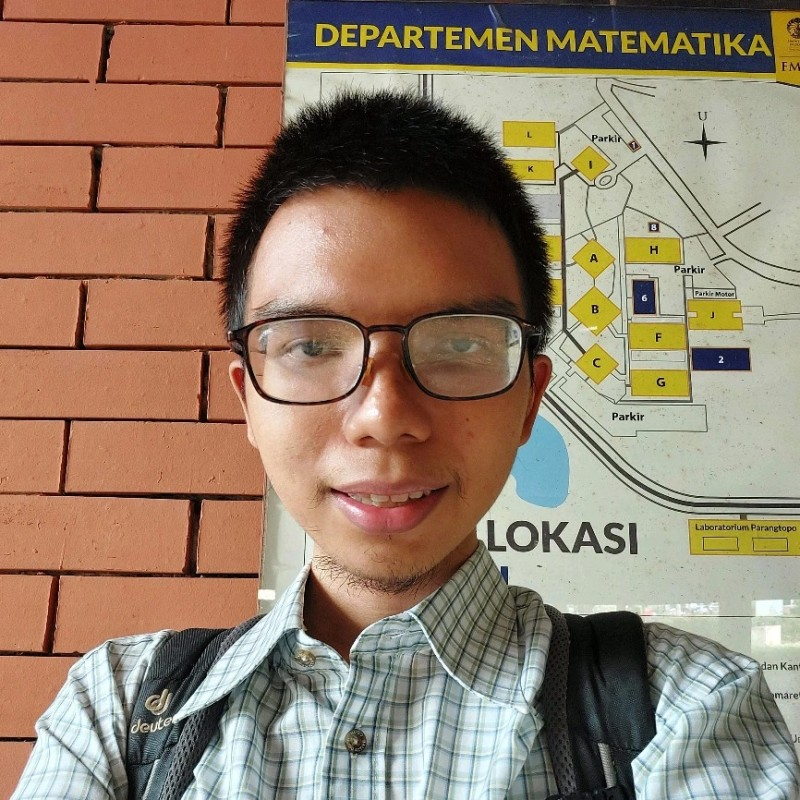
\includegraphics[height=4cm, width=4cm]{profile_pic.jpeg}
        \end{tabular}
        &
        \begin{tabular}{l}
            \parbox{0.5\linewidth}{%  change the parbox width as appropiate
            \begin{itemize}
                \item Undergraduate Final Year Mathematics Student at University of Indonesia
                \item Interests:
                \begin{itemize}
                    \item Reliable and verified systems
                    \item Building technology to help make people's lives easier
                    \item Mathematics and its applications
                \end{itemize}
            \end{itemize}
            }
        \end{tabular}
    \end{tabular}
    % ref: https://tex.stackexchange.com/questions/165475/figure-next-to-text-in-beamer
\end{frame}

\begin{frame}{Daftar Isi}
    \tableofcontents
\end{frame}

\section{Haskell untuk \textit{Backend}}

\begin{frame}[fragile]{\textit{Type Alias}}
\begin{minted}{haskell}
type HourNum = Int
type DayNum = Int
type DayHour = (DayNum, HourNum)

type WorkCalendar = [DayHour]
type FullHours = [DayHour]
type DayHourNum = Int

...
\end{minted}
\end{frame}

\begin{frame}[fragile]{Maybe, \textit{Higher-Order Function}}
\begin{minted}{haskell}
getDayHourToFromNum
:: WorkCalendar -> FullHours
-> (DayHour -> Maybe DayHourNum, DayHourNum 
-> Maybe DayHour)
getDayHourToFromNum wcInput fhInput = (f, fInv)
    where
        wc = (nub . sort) wcInput
        fh = (nub . sort) fhInput
        filtered = filter (`notElem` fh) wc
        listDayHourIdx = getPairsObjIdx filtered
        f = listToMaybeFunction listDayHourIdx
        fInv = (listToMaybeFunction . revTuplesInList)
            listDayHourIdx
\end{minted}
\end{frame}

\section{Haskell untuk \textit{Frontend}}

\begin{frame}{Reflex}
    \begin{itemize}
        \item Teknologi yang digunakan untuk \textit{frontend}: Reflex, \textit{framework} di Haskell
        \item Paradigma \textit{functional reactive programming} (FRP) yang menjunjung tinggi pemrograman fungsional dan juga cepat
        \item Semuanya tetap \textit{purely functional} semaksimal mungkin
    \end{itemize}
\end{frame}

\begin{frame}[fragile]{Penggunaan \textit{Applicative Functor}}
\begin{minted}{haskell}
el "h2" $ text "Tasks"
...
el "p" $ text "Example: [(\"task1\",
    (1,4), 1), (\"task2\", (2,3), 2)]"
taskListInput <- textArea def
let hts = fromMaybe tempHumanTasks . 
          readMaybe . T.unpack <$>
          value taskListInput
el "p" $ text "Value received:"
display hts
\end{minted}
\end{frame}

\section{Demo dan Dokumentasi}

\begin{frame}{Dokumentasi}
    \url{https://github.com/BismaBRJ/human-task-scheduler-genetic-algo-hs}

    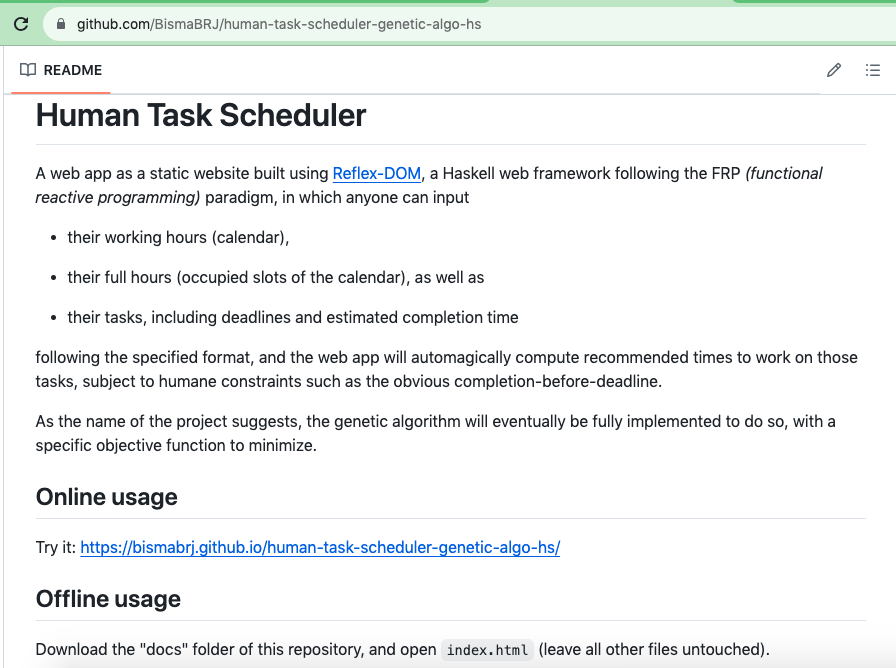
\includegraphics[scale=0.4]{dokumentasi.png}
\end{frame}

\begin{frame}{Demo}
    \url{https://bismabrj.github.io/human-task-scheduler-genetic-algo-hs/}

    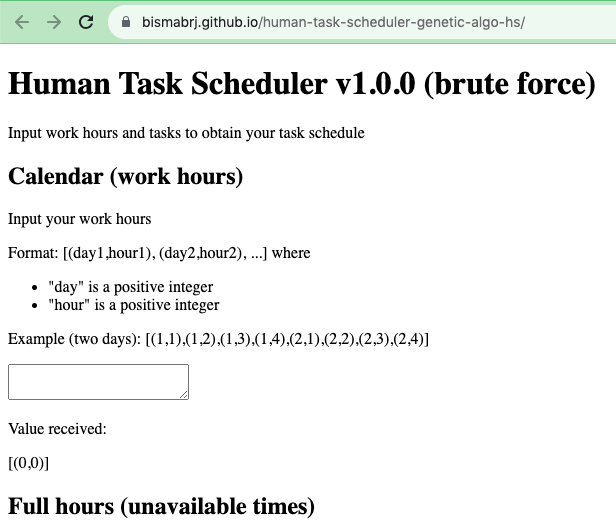
\includegraphics[scale=0.4]{demo.png}
\end{frame}

\begin{frame}{Beberapa \textit{Lessons Learned}}
    \begin{enumerate}
        \item Berbagai fitur pemrograman fungsional sangat bermanfaat, tidak hanya untuk yang umum dikenal di ranah akademis
        \item Haskell kurang digunakan terutama untuk pemrograman web, padahal bisa mengurangi \textit{error}
    \end{enumerate}
\end{frame}

\end{document}